\documentclass[8pt, a4paper]{article}
\usepackage{geometry}
\geometry{total={170mm, 257mm},left=20mm, top=20mm}
\usepackage{graphicx}


\begin{document}
\setlength \topmargin{-1in}
\title{\textbf{Software Engineering for Distributed and Interactive Systems.}}
\author{\textbf{James Ravenhill}}
\date{}
\maketitle

\section{Introduction} 

//// summarise the project, list objectives, outlines the structure of the documentation.


\section{Design}
\begin{figure}[h]
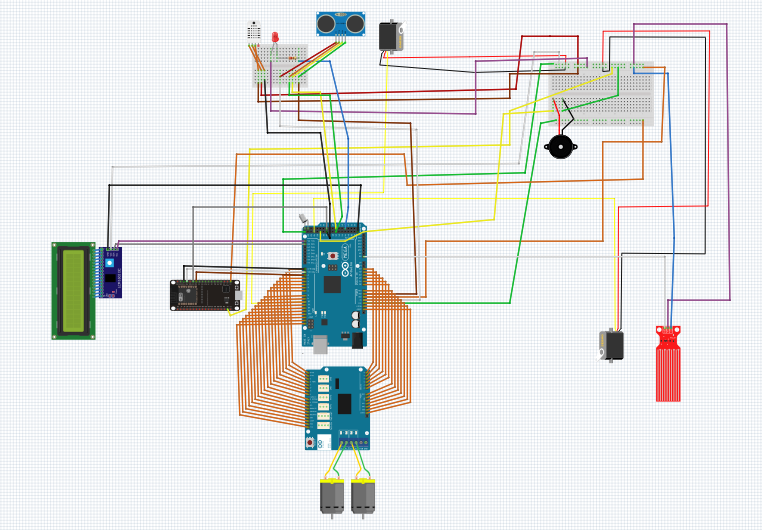
\includegraphics[height=5cm, width=7.5cm]{schematic}
\centering
\end{figure}

\section{Implementation}


\section{Testing}

\section{Evaluation}


\section{Code quality/remarks} ////this may get cut if needed as in more an non written task
////discuss multi and single core methods in a ReadMe file!!!


\section{Demonstration}
////film the video and then refer to it for the following subsections


\subsection{Distribution}
///Define what a distributed system is 

\subsection{Interactive}
///Define what an interactive system is

\subsection{Performance}






\section{Conclusion}


\section{Reference Library and appendices}




\end{document}